\documentclass[tikz,border=0pt]{standalone}
\usepackage[american]{circuitikz}
\usetikzlibrary{arrows.meta,calc,positioning,decorations.pathmorphing,patterns}
\definecolor{zyloTeal}{HTML}{174A5B}
\definecolor{zyloTealTwo}{HTML}{246B7A}
\definecolor{zyloInk}{HTML}{1F2933}
\definecolor{zyloSoft}{HTML}{EAF4F4}
\definecolor{zyloPaper}{HTML}{F8FAFB}
\definecolor{zyloLine}{HTML}{44606B}
\definecolor{zyloOrange}{HTML}{D97706}
\begin{document}
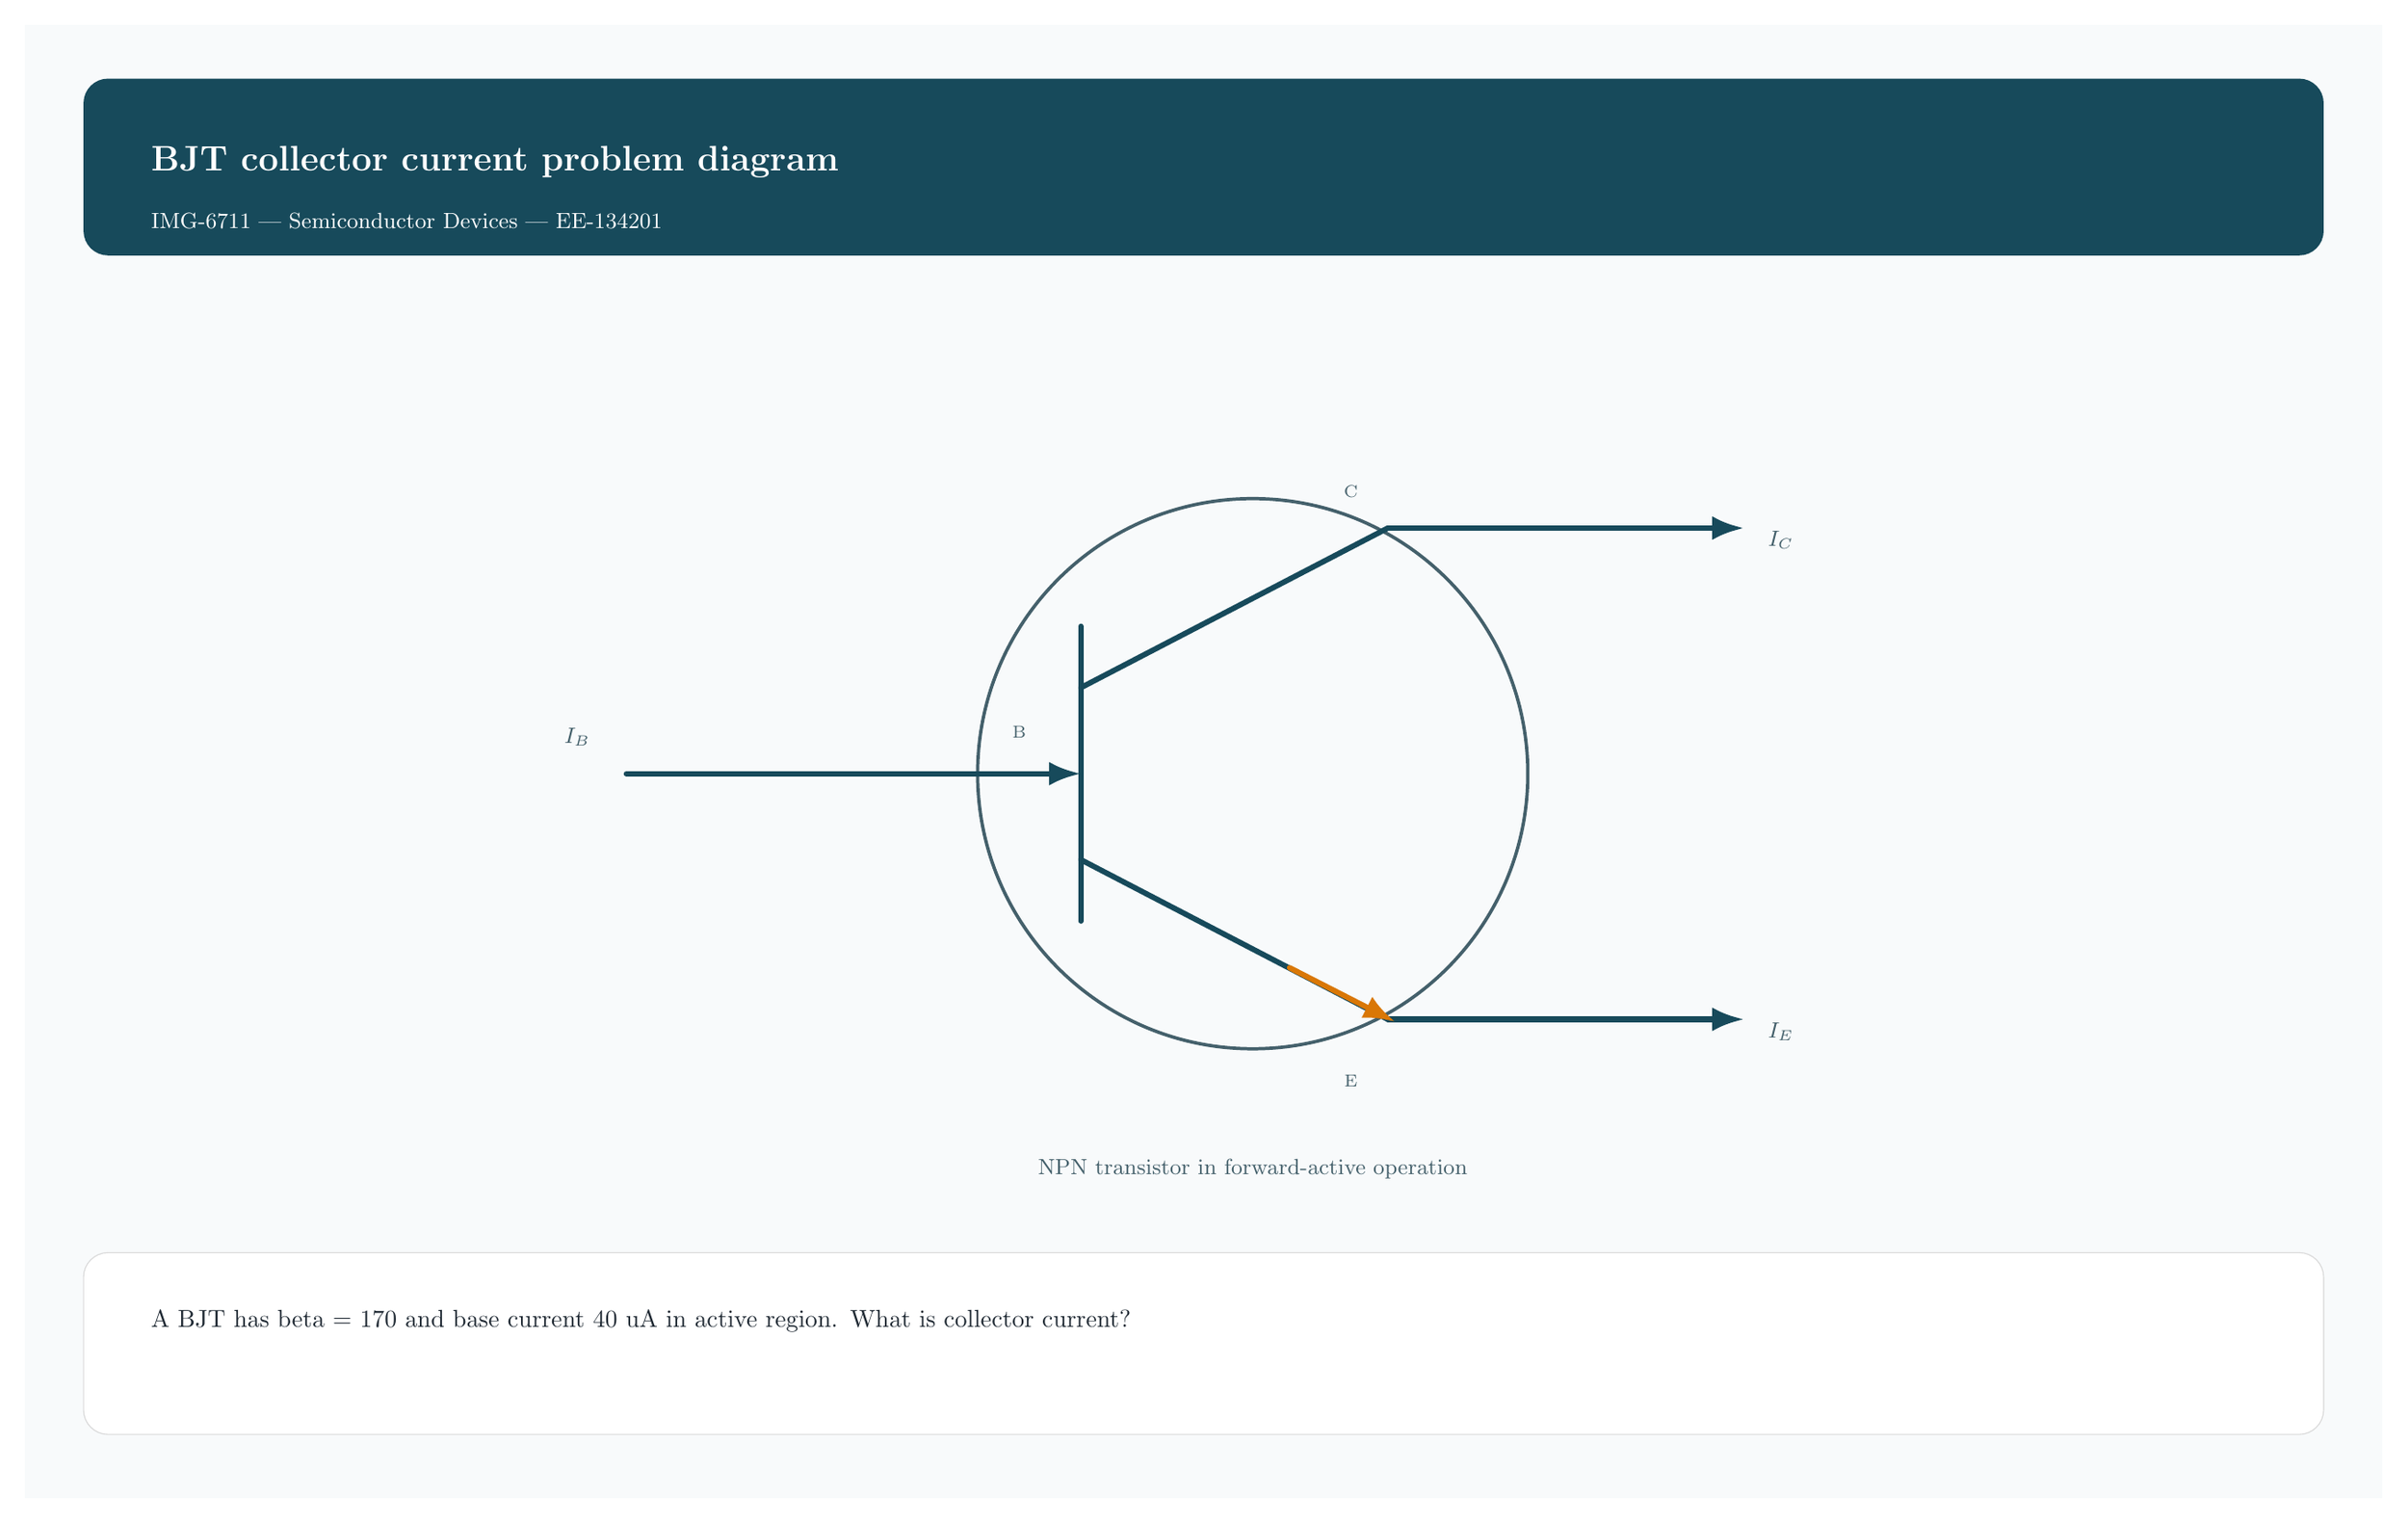
\begin{tikzpicture}[x=1pt,y=-1pt,>=Latex,line cap=round,line join=round]
\path[fill=zyloPaper] (0,0) rectangle (960,600);
\path[fill=zyloTeal,rounded corners=10pt] (24,22) rectangle (936,94);
\node[anchor=west,text=white,font=\bfseries\Large] at (48,56) {BJT collector current problem diagram};
\node[anchor=west,text=white!82,font=\small] at (48,80) {IMG-6711 | Semiconductor Devices | EE-134201};
\tikzset{wire/.style={draw=zyloTeal,line width=2.2pt},thinwire/.style={draw=zyloLine,line width=1.35pt},accent/.style={draw=zyloOrange,line width=2.2pt},box/.style={draw=zyloTealTwo,fill=zyloSoft,line width=1.5pt,rounded corners=8pt}}
\draw[thinwire] (500,305) circle (112); \draw[wire] (430,245) -- (430,365);
\draw[wire,->] (245,305) -- (430,305); \draw[wire] (430,270) -- (555,205); \draw[wire,->] (555,205) -- (700,205);
\draw[wire] (430,340) -- (555,405); \draw[wire,->] (555,405) -- (700,405); \draw[accent,->] (515,384) -- (558,406);
\node[font=\small,text=zyloLine] at (225,290) {$I_B$}; \node[font=\small,text=zyloLine] at (715,210) {$I_C$}; \node[font=\small,text=zyloLine] at (715,410) {$I_E$};
\node[font=\scriptsize,text=zyloLine] at (405,288) {B}; \node[font=\scriptsize,text=zyloLine] at (540,190) {C}; \node[font=\scriptsize,text=zyloLine] at (540,430) {E};
\node[font=\small,text=zyloLine] at (500,466) {NPN transistor in forward-active operation};
\path[draw=black!15,fill=white,rounded corners=10pt] (24,500) rectangle (936,574);
\node[anchor=west,text width=860pt,align=left,text=zyloInk,font=\normalsize] at (48,528) {A BJT has beta = 170 and base current 40 uA in active region. What is collector current?};
\end{tikzpicture}
\end{document}
